% Chapter Template

\chapter{Results - Sliding Puzzle} % Main chapter title

\label{sec:ResultsSP} % Change X to a consecutive number; for referencing this chapter elsewhere, use \ref{ChapterX}





\begin{center}
\begin{tabular}{l*{9}{c}r}
\hline
\textbf{solver}      & & \textbf{Sliding Puzzle} & \textbf{2x2} & \textbf{2x3} & \textbf{2x4} & \textbf{2x5}  & \textbf{3x3} & \textbf{3x4} & \textbf{4x4} \\ 
\hline
BFS   & & & & & & &  x  & & \\
\hline
A$^{*}$[Manhattan]   & & & & & & &  x  & & \\
\hline
A$^{*}$[Manhattan++]   & & & & & & &  x  & & \\
\hline
A$^{*}$[Perfect]   & & &  x  &  x  &  x  &  x  &  x  & & \\
\hline
Naive   & & & & & & &  x  & & \\
\hline
A$^{*}$[DL[A$^{*}$[Perfect]]]   & & & & & & &  x  & & \\
\hline
A$^{*}$[DRL]   & & & & & & &  x  & & \\
\hline
A$^{*}$[DQL]   & & & & & & &  x  & & \\
\hline
MCTS[DQL][c=TBD]   & & & & & & &  x  & & \\
\end{tabular}
\end{center}












%----------------------------------------------------------------------------------------
%	SECTION 1
%----------------------------------------------------------------------------------------

\section{Low dimension}
\label{sec:SPLowDimension}

\subsection{God numbers and hardest puzzles}

As mentioned in chapter \ref{sec:Puzzles}, the state space cardinality for the SP grows very quickly with n and m. Here are the only dimensions which have less than 239.5 millions states. Note I am also only considering n $\leq$ m since (p, q) can always be solved if we know how to solve (q, p):
\\
\\
\begin{center}
\begin{tabular}{l*{6}{c}r}
n              & m & 2 & 3 & 4 & 5\\
\hline
2              &   & 12 & 360 & 20,160 & 1,814,400 \\
3              &   &   & 181,440 &  &    \\
\end{tabular}
\end{center}
In this section, I will discuss \textbf{full} results for these 5 puzzles. In order to fully solve them, one can simply use rubiks.scripts.learner, setting up the PerfectLearner with A* and manhattan heuristic, or instantiate directly a PerfectLearner as have seen in section \ref{PLSS}
I obtained the following God numbers for these puzzles:
\begin{center}
\begin{tabular}{l*{6}{c}r}
n              & m & 2 & 3 & 4 & 5\\
\hline
2              &   & 6 & 21 & 36 & 55* \\
3              &   &   & 31 &  &    \\
\end{tabular}
\end{center}
* provisional result
\\
\\
Notice that among the above dimensions, (n=2, m=5) is the largest and hardest one. I had to run its PerfectLearner over a couple of days, on a c5.18xlarge instance (72 cores) on Amazon EC2.
\\
\\
The perfectLearner also keeps track of (one of) the hardest puzzles it has encountered (i.e. requiring a number of steps equal to their respective God number to solves):
\\
\\
\underline{Most difficult 2x2 (6 moves)}:
\begin{center}
\begin{three}
\setrow{2}{,3}
\setrow{1}{2,1}
\end{three}
\end{center}
\underline{Most difficult 2x3 (21 moves)}:
\begin{center}
\begin{five}
\setrow{2}{4,5,}
\setrow{1}{1,2,3}
\end{five}
\end{center}
\underline{Most difficult 2x4 (36 moves)}:
\begin{center}
\begin{seven}
\setrow{2}{,7,2,1}
\setrow{1}{4,3,6,5}
\end{seven}
\end{center}
\underline{Most difficult 2x5 (55* moves)}:
\begin{center}
\begin{nine}
\setrow{2}{,9,3,7,1}
\setrow{1}{5,4,8,2,6}
\end{nine}
\end{center}
* provisional result
\\
\\
\underline{Most difficult 3x3 (31 moves)}:
\begin{center}
\begin{eight}
\setrow{3}{8,6,7}
\setrow{2}{2,5,4}
\setrow{1}{3,,1}
\end{eight}
\end{center}




\subsection{Manhattan heuristic}
\label{MHComp}
In this section, I verify empirically that, as expected, the overhead of adding penalty in Manhattan++ for the linear constraint (which have all been precomputed and stored in a database) is more than compensated for by the reduction in nodes expansion. I have run my solver script for (n=2, m=5) in performance test mode, for both Manhattan and Manhattan++, with 250 randomly shuffled puzzles with \textit{nb\_shuffles} from 0 to 60 by increment of 5, as well as with \textit{nb\_shuffles = $\inf$}. The resulting run time and nodes expansions are as follows:

\begin{figure}[H]
\centering
\hspace*{-2.5cm}
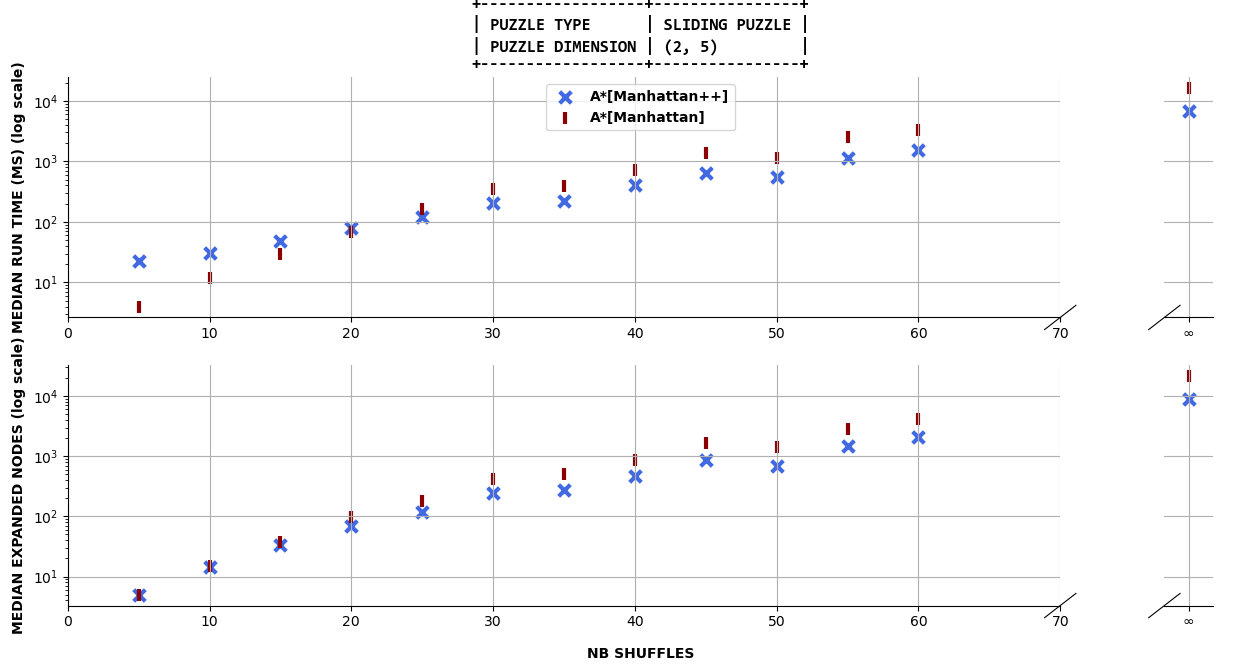
\includegraphics[scale=0.45]{./Figures/25SPPerformanceManhattan}
%\decoRule
\caption[SP]{Manhattan vs Manhattan++}
\label{fig:25SPPerformanceManhattan}
\end{figure}

As can be seen, for low difficulty (up to \textit{nb\_shuffles = 20}), the node expansions are about the same in both cases, and the overhead of adding the linear constraints penalty increases the run time. However, for any non trivial case, Manhattan++ outperforms considerably (by a factor of about 2.5). For the 250 \textit{perfectly} shuffled instances, I got the following:



\begin{center}
\begin{tabular}{l*{7}{c}r}
                              & avg cost  & max cost & avg nodes & max nodes & avg run time (ms) & max run time (ms) \\
\hline
Manhattan                   &  34.7  & 50 & 133,332 & 2,110,887 & 49,561 & 606,838 \\
Manhattan++              & 34.7 &  50 & 53,637 & 962,324 & 19,723 & 239,468 \\
Improvement               & n/a &  n/a & x2.5 & x2.2 & x2.5 & x2.5 \\
\end{tabular}
\end{center}



%-----------------------------------
%	SECTION 2
%-----------------------------------
\section{Intermediary case - 3x3}
\label{sec:S33}


\subsection{Perfect learner}
As discussed in the previous section section \ref{sec:SPLowDimension}, the 3 by 3 SP is one of the cases I have been able to solve perfectly, since it only has 181,440 possible configurations. Its God number is only 31, which definitely makes it manageable. However, this is already an intermediary size, large enough that it is worth trying and comparing a few different methods, including deep reinforcement learning. To start with, I ran the PerfectLearner with n=m=3, and the results are shown below in figure \ref{fig:33SPPerfectLearning}. It is interesting to note that there are only two hardest configurations (cost 31) and 221 configurations of cost 30.


\newgeometry{top=0mm, bottom=0mm, left=0mm, right=0mm}
\begin{landscape}
\centering\vspace*{\fill}
\begin{figure}[H]
\centering
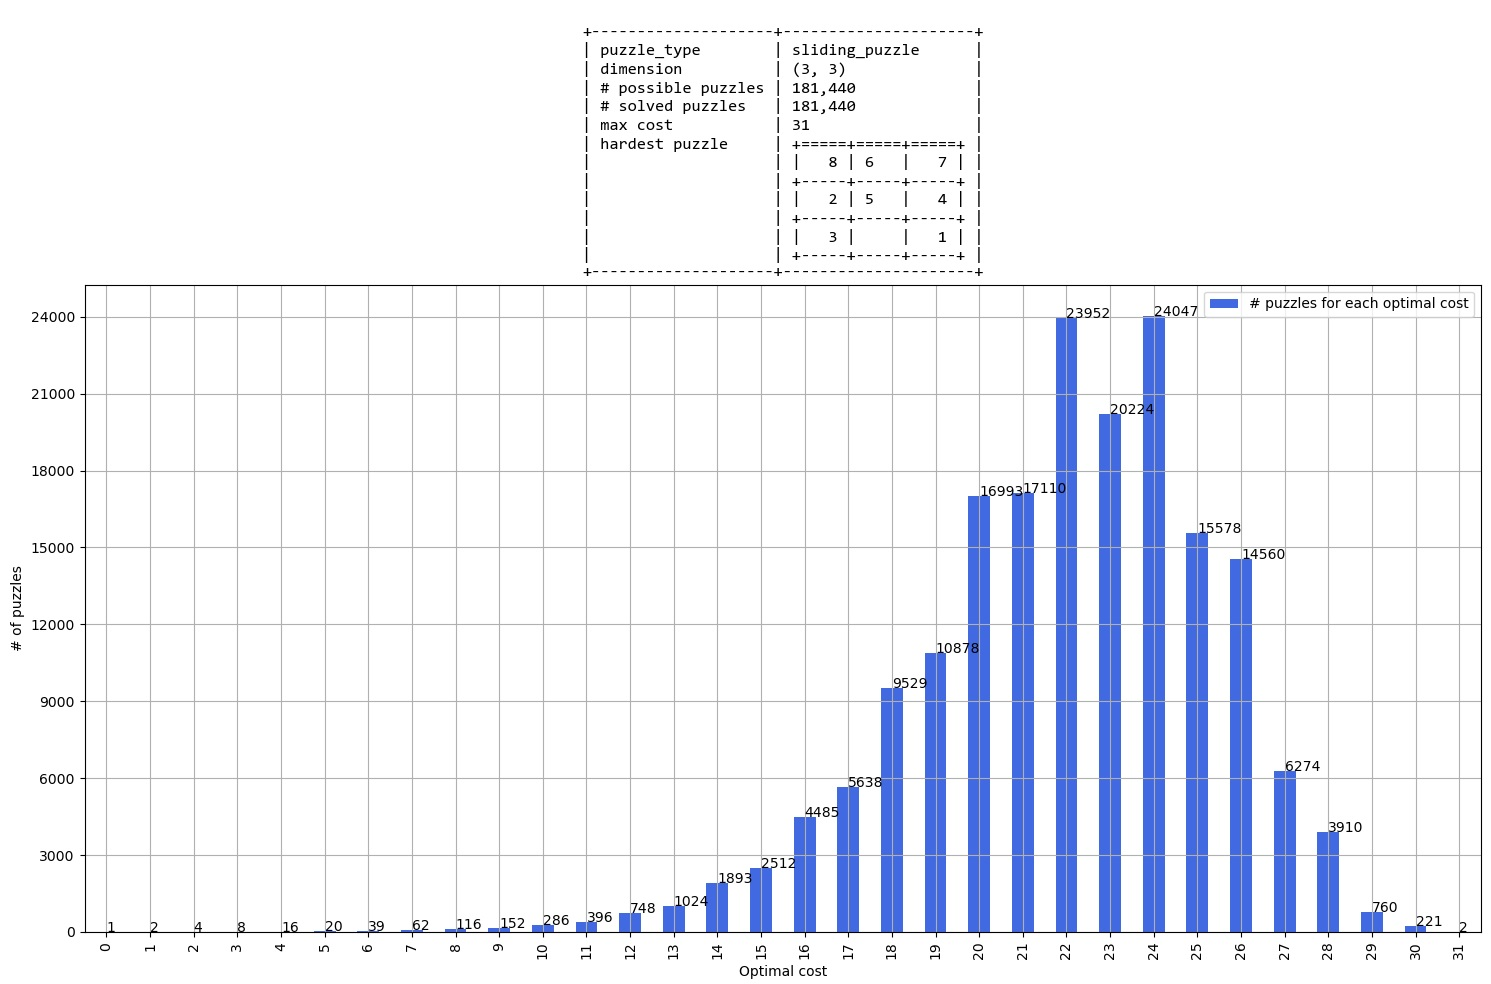
\includegraphics[scale=0.7]{./Figures/33SPPerfectLearning.jpeg}
%\decoRule
\caption[33SPPerfectLearning]{Perfect Learning 3x3 SP}
\label{fig:33SPPerfectLearning}
\end{figure}
\vfill
\end{landscape}
\restoregeometry




\subsection{Deep reinforcement learner}
 The DeepReinforcementLearner's learning is shown in figure \ref{fig:33SPDeepReinforcementLearning}:

\newgeometry{top=0mm, bottom=0mm, left=0mm, right=0mm}
\begin{landscape}
\centering\vspace*{\fill}
\begin{figure}[H]
\centering
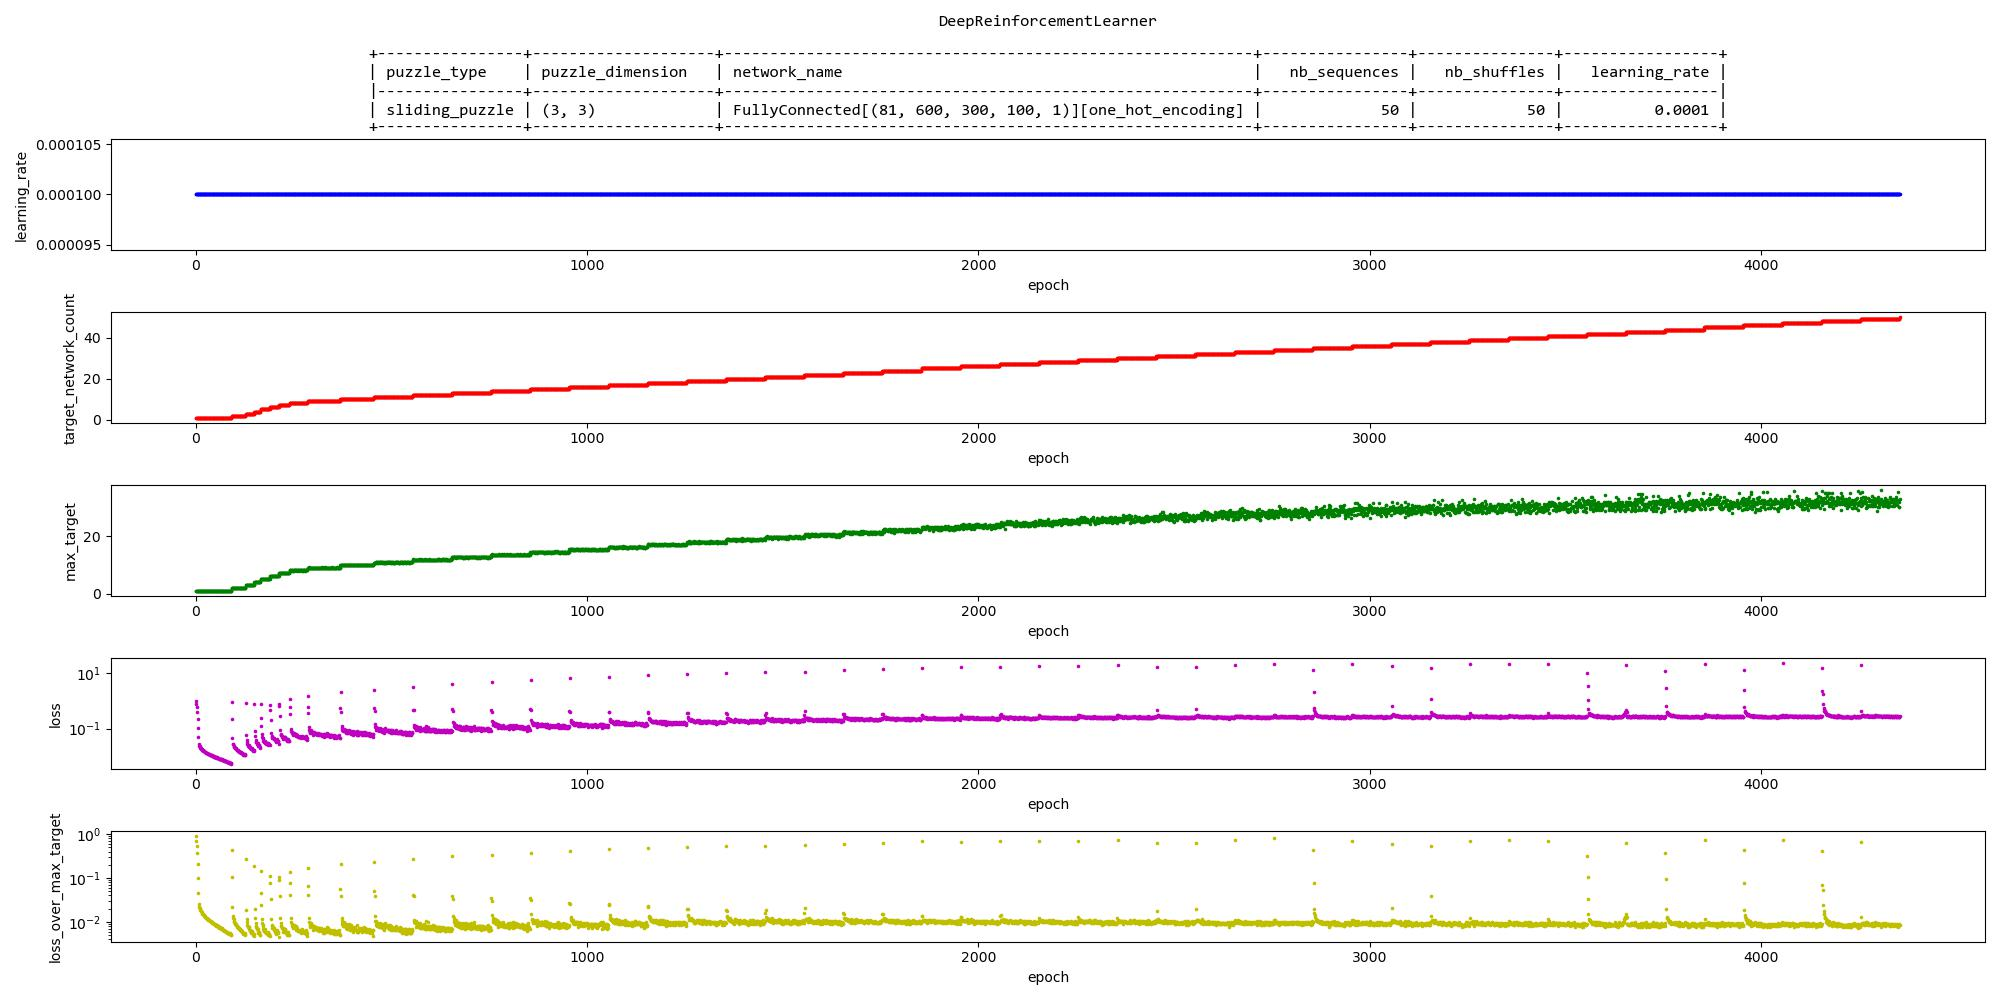
\includegraphics[align=c, scale=0.55]{./Figures/33SPDeepReinforcementLearning.jpeg}
\caption[33SPDeepReinforcementLearning]{Deep reinforcement learner 3x3 SP}
\label{fig:33SPDeepReinforcementLearning}
\end{figure}
\vfill
\end{landscape}
\restoregeometry


\subsection{Solvers' comparison}
\label{ssec:33SPSC}
Let me discuss a comparison of several algorithms on 1000 random puzzles generated for a number of random shuffling (with best-effort-no-backtracking) from 0 to 50 in step of 2, as well as for perfect shuffling (denoted by $\infty$) on the comparison graphs. The results are shown in figure \ref{fig:33SPPerformance}

\newgeometry{top=0mm, bottom=0mm, left=0mm, right=0mm}
\begin{landscape}
\centering\vspace*{\fill}
\begin{figure}[H]
\centering
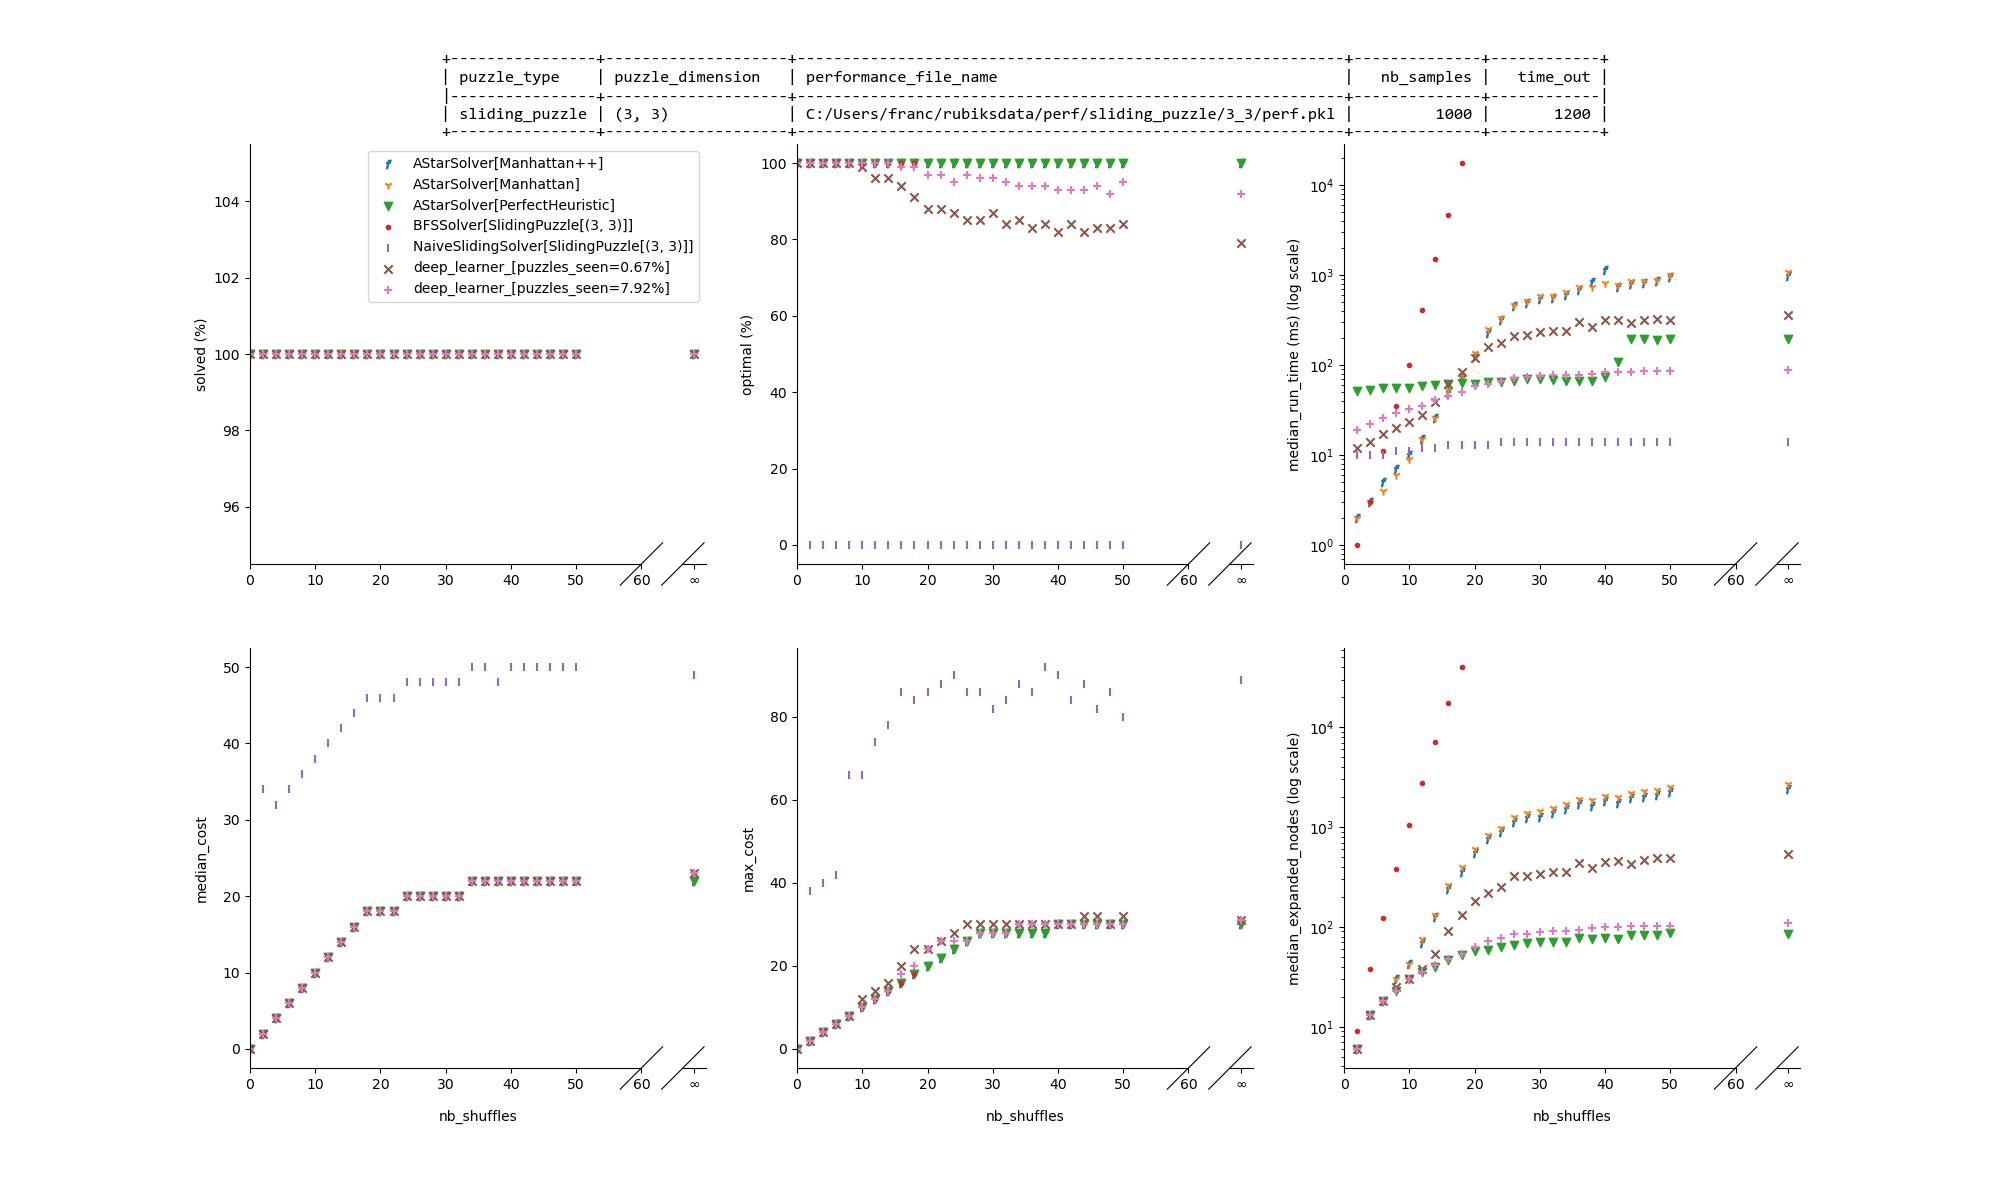
\includegraphics[scale=0.63]{./Figures/33SPPerformance.jpeg}
%\decoRule
\caption[33SPPerformance]{Solvers' performance comparison 3x3 SP}
\label{fig:33SPPerformance}
\end{figure}
\vfill
\end{landscape}
\restoregeometry


\subsection{Solving the hardest 3x3 problem}
To finish with the 3x3 SP, let me try to throw one of the two hardest 3x3 configurations (see subsection \ref{sec:SPLowDimension}) at the different solvers to see how they fare. The results are shown here

\begin{center}
\begin{tabular}{l*{5}{c}r}
\hline
\textbf{solver}      & & \textbf{cost} & \textbf{\# expanded nodes} & \textbf{run time (ms)} \\
\hline
AStarSolver[Manhattan]   &   &      31  & 58,859  & 11,327  \\
\hline
AStarSolver[Manhattan++]   &   &      31  & 34,224  & 7,080  \\
\hline
AStarSolver[PerfectHeuristic]  &   & 31 & 1,585 & 202 \\
\hline
AStarSolver[DRLHeuristic]  &   & 31 & 101 & 58 \\
\hline
MCTSSolver[DQLHeuristic][c=0]  &   & 101 & 103 & 456 \\
\hline
MCTSSolver[DQLHeuristic][c=69]  &   & 35 & 2,244 & 8,873 \\
\hline
BFS  &   & - & - & time out \\
\hline
NaiveSlidingSolver  &   & 61 & n/a & 18 \\
\hline
\end{tabular}
\end{center}
On this specific configuration, there was obviously no chance that the BFS would complete, hence it timed out. It would have no matter what time out I set. Indeed, since it has no heuristic to guide its search, it would need to explore in the order of $3^{31}$ - roughly 617 trillions - nodes to reach the goal!
\\
Rather interestingly, my DRL heuristic performs much better than the manhattan heuristic (not super suprising), but also outperforms the perfect heuristic quite significantly both in terms of run time and of nodes expansion. Obviously there is no guarantee that the perfect heuristic will not be outperformed on some random configuration, and it does on this occasion. However, as we have seen in the previous subection \ref{ssec:33SPSC}, it is not the case on average.
\\
Finally, the naive solver outperforms every other solver in terms of run time, but finds a rather poor solution of 61 moves.



%-----------------------------------
%	SECTION 3
%-----------------------------------
\section{3x4}

\label{ssec:34SPSC}

\newgeometry{top=0mm, bottom=0mm, left=0mm, right=0mm}
\begin{landscape}
\centering\vspace*{\fill}
\begin{figure}[H]
\centering
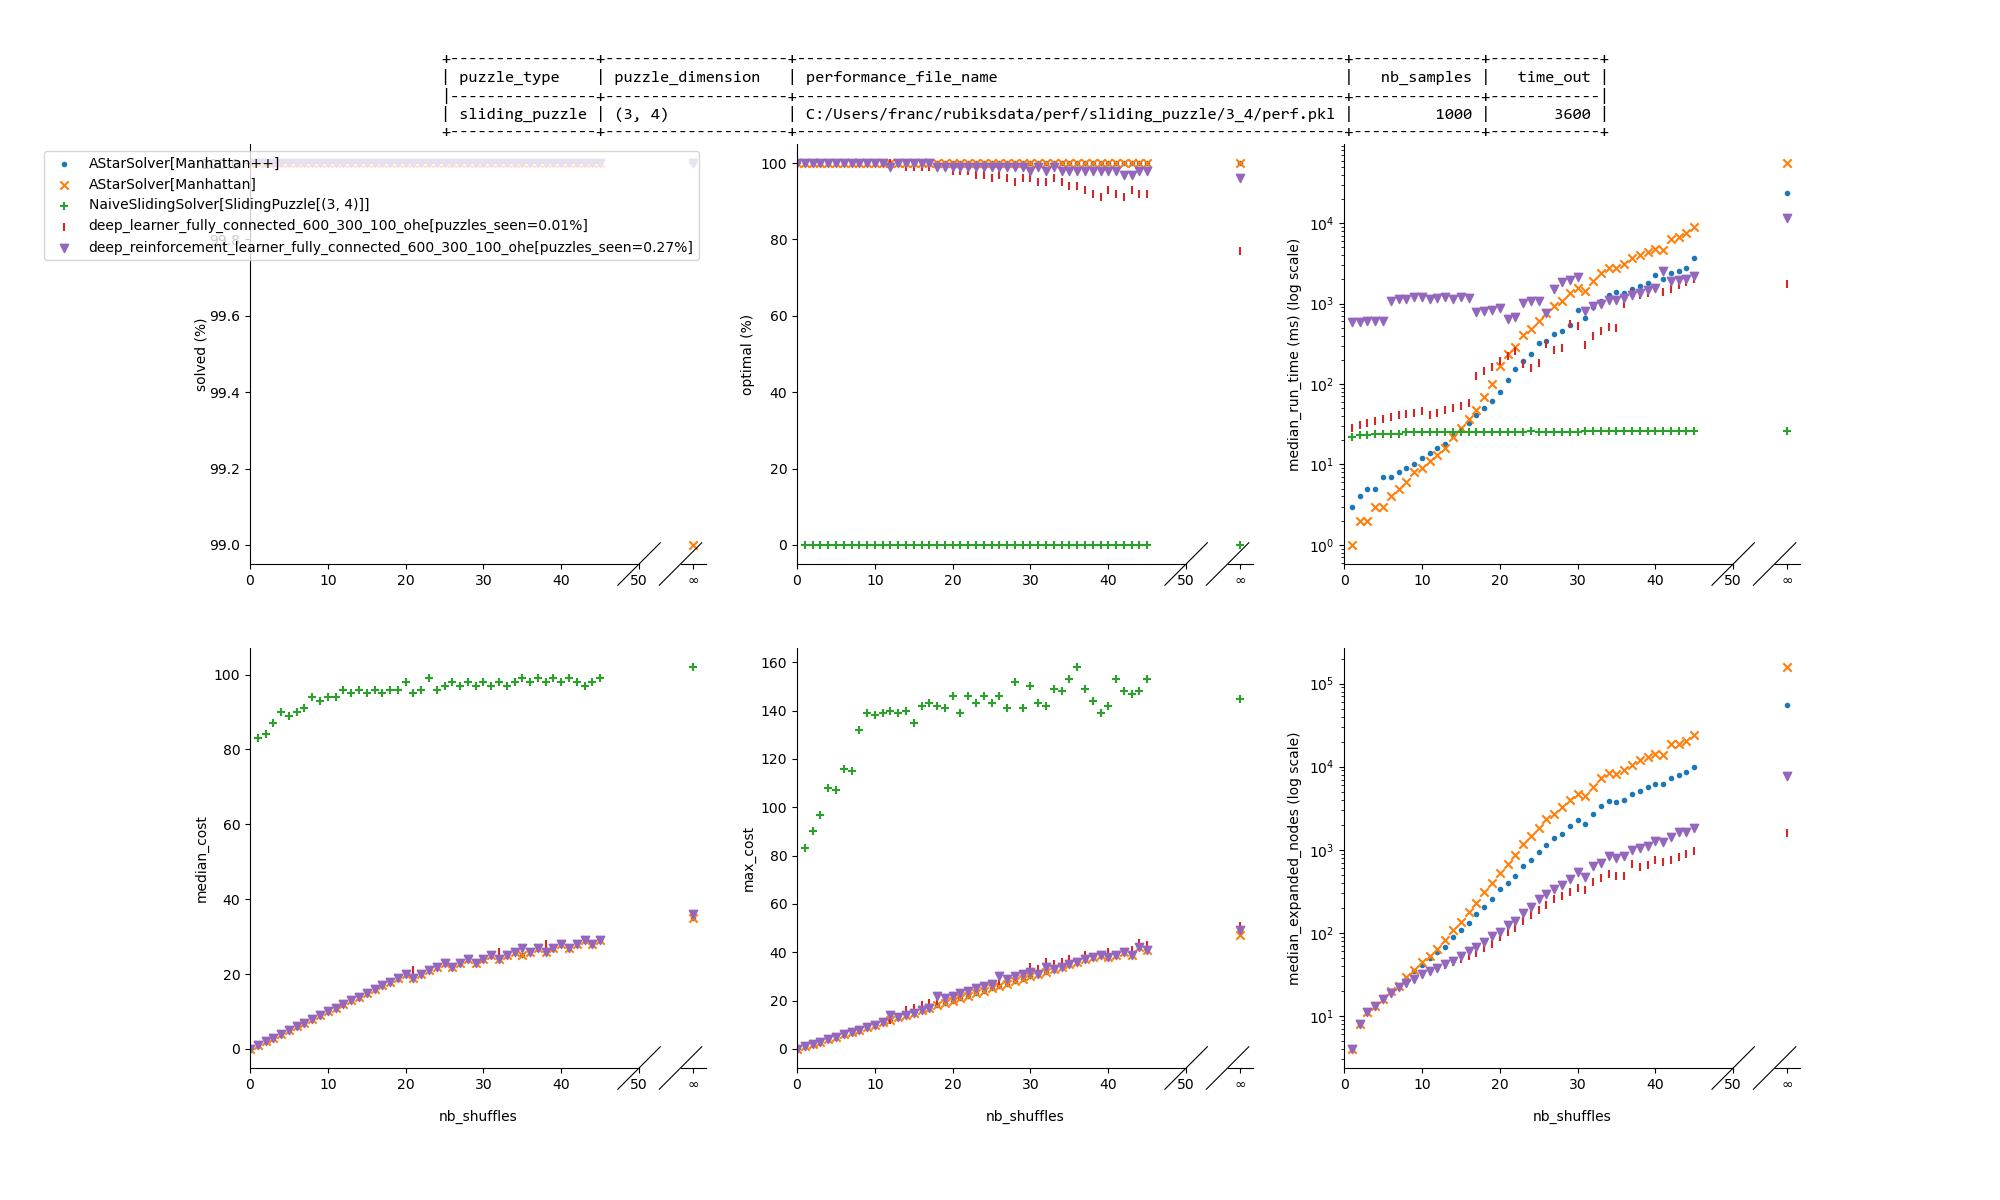
\includegraphics[scale=0.63]{./Figures/34SPPerformance.jpeg}
%\decoRule
\caption[34SPPerformance]{Solvers' performance comparison 3x4 SP}
\label{fig:34SPPerformance}
\end{figure}
\vfill
\end{landscape}
\restoregeometry
%-----------------------------------
%	SECTION 4
%-----------------------------------

\section{4x4}



\label{ssec:44SPSC}

\newgeometry{top=0mm, bottom=0mm, left=0mm, right=0mm}
\begin{landscape}
\centering\vspace*{\fill}
\begin{figure}[H]
\centering
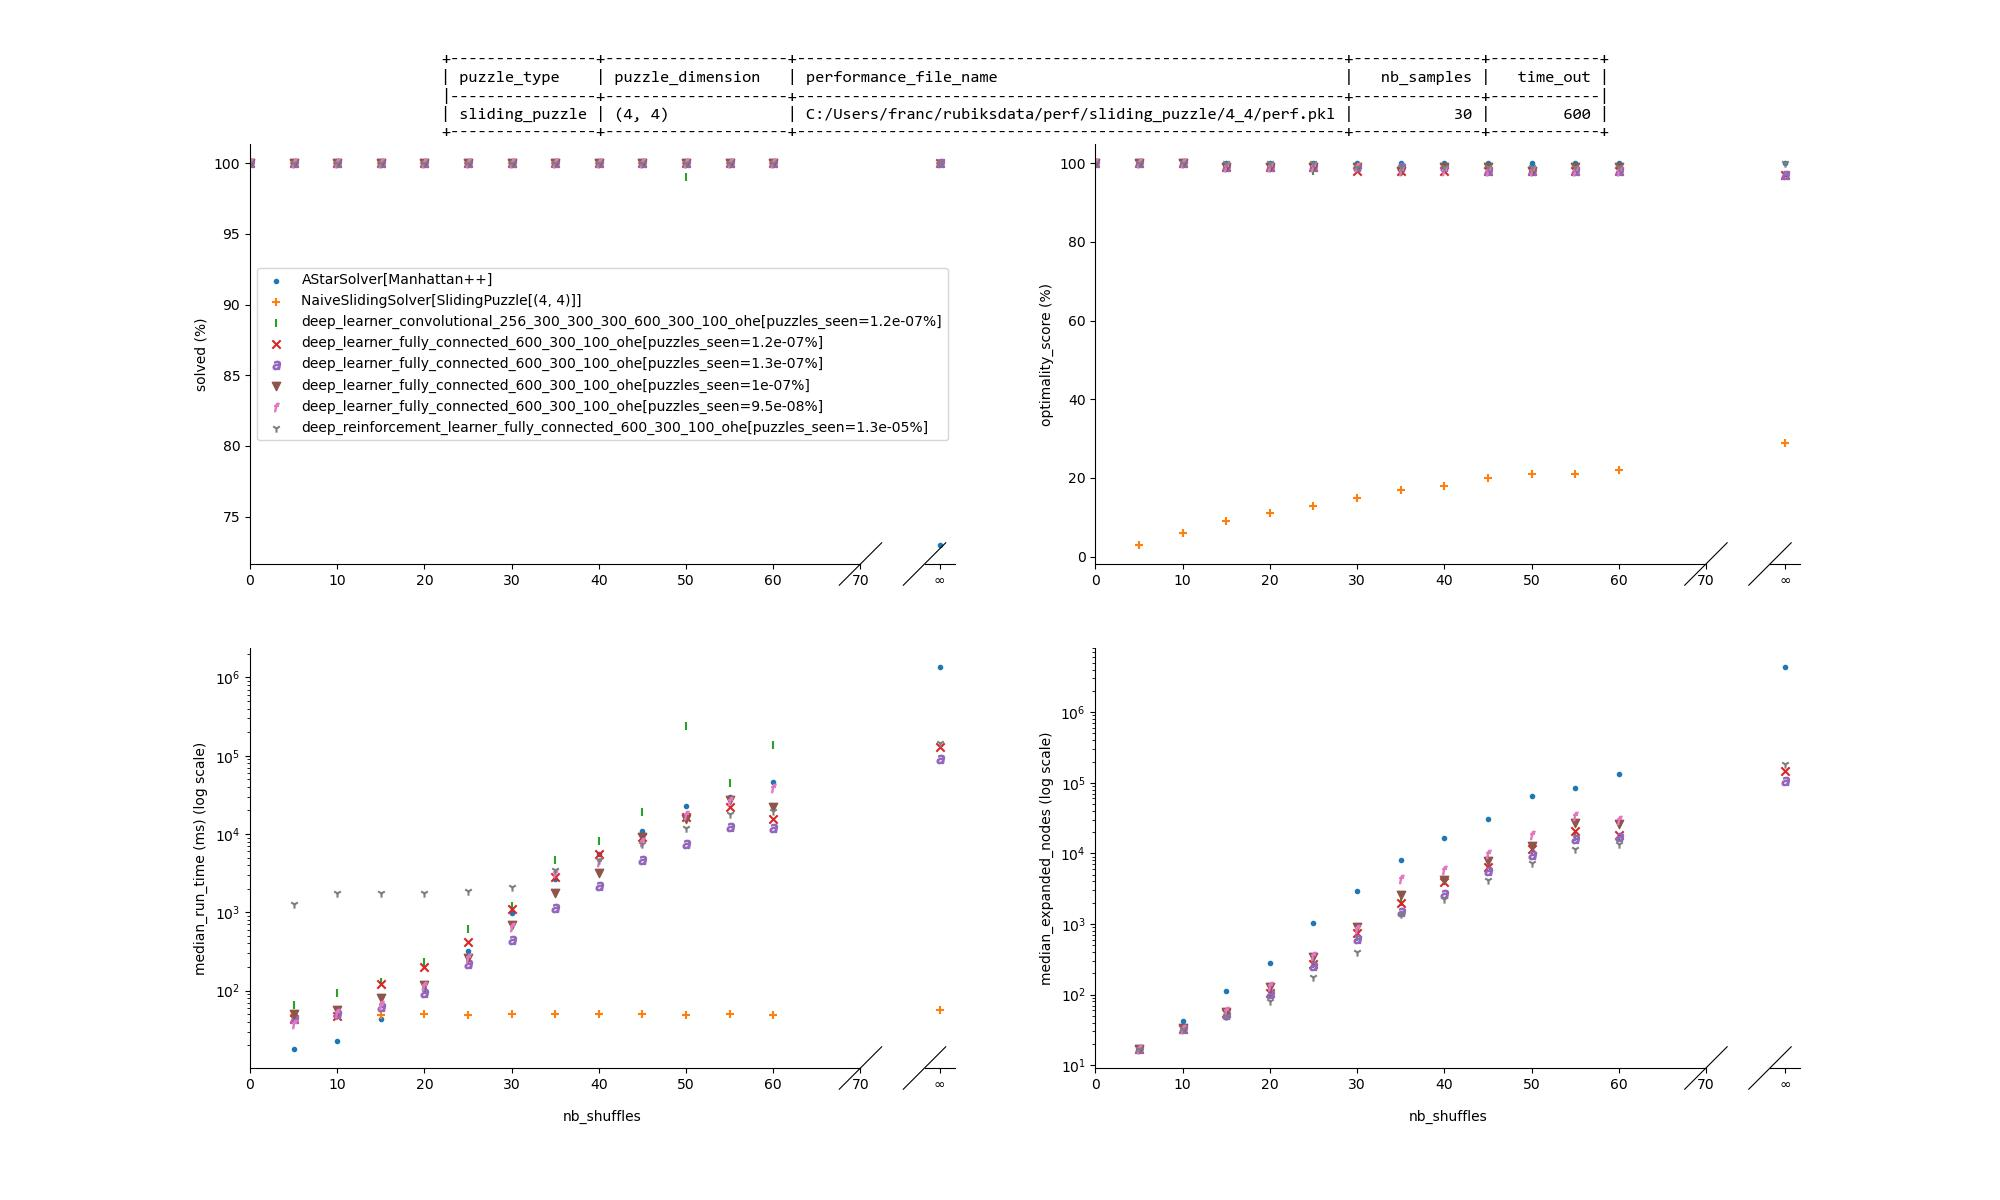
\includegraphics[scale=0.63]{./Figures/44SPPerformanceAll.jpeg}
%\decoRule
\caption[44SPPerformance]{Solvers' performance comparison 4x4 SP}
\label{fig:44SPPerformance}
\end{figure}
\vfill
\end{landscape}
\restoregeometry

%-----------------------------------
%	SECTION 5
%-----------------------------------

\section{5x5}

TBD
